\subsection{Fashion-MNIST: khai thác mẫu trực quan}
\label{sec:fashion}
\subsubsection{Bài toán và phạm vi ứng dụng}
Eclat nhận tập item rời rạc, còn ảnh là một lưới pixel có cấu trúc không
gian. Quyết định chính là chuyển ảnh thành giao dịch mà vẫn truy vết
được item về ảnh gốc. Nhóm dùng túi từ thị giác
(\textit{Bag of Visual Words}, BoVW)~\cite{Sivic03}: mỗi vùng ảnh nhỏ được
gán một visual word, rồi tập mã xuất hiện trong ảnh trở thành giao dịch.
Frequent itemset mô tả tổ hợp visual words thường cùng xuất hiện.

Fashion-MNIST~\cite{Xiao2017} gồm 60.000 ảnh train và 10.000 ảnh test,
mỗi ảnh xám $28\times28$ pixel, chia đều cho mười lớp. Mỗi lớp có 6.000
ảnh train và 1.000 ảnh test. Các lớp gồm T-shirt/top, Trouser, Pullover,
Dress, Coat, Sandal, Shirt, Sneaker, Bag và Ankle boot. Nhãn được giữ
riêng để mô tả kết quả sau mining, không đưa vào descriptor hay tập item.

Bài toán hiện tại là phân tích mô tả, không phải huấn luyện bộ phân loại.
Profile release cố định B0/K32/seed123/S0 và dùng toàn bộ 70.000 ảnh để
học từ điển. Đây là baseline được chọn cho luồng release; chưa có cơ sở
gọi nó là cấu hình tối ưu qua EDA2. Lưới K/seed và spatial encoding là
thí nghiệm riêng, không nhập vào kết quả của profile cố định này.

\subsubsection{Kiểm định dataset và định danh ảnh}
Pipeline tải hoặc dùng lại bốn archive ảnh/nhãn chính thức, đối chiếu
SHA-256, giải nén gzip và đọc IDX. Kiểm tra magic number, số ảnh/nhãn,
kích thước 28$\times$28 và nhãn trong $0{:}9$ giúp phát hiện archive hỏng
hoặc sai bộ dữ liệu. Không chỉ dựa vào tên file hoặc việc giải nén thành
công để xác nhận đúng dữ liệu.

Một ảnh có ID ổn định dạng \texttt{train:<index>} hoặc
\texttt{test:<index>}, với index nguồn bắt đầu từ 0. TID của database bắt
đầu từ 1 và là thứ tự giao dịch, không phải nhãn lớp hoặc mã ảnh. Phân
biệt này tránh nhầm chỉ số mảng Julia bắt đầu từ 1 với vị trí nguồn IDX.
Hai ảnh khác nhau có giao dịch giống nhau vẫn giữ hai TID riêng.

Notebook đầu ghi dataset manifest gồm run ID, số ảnh, shape và hash
archive. Các bước sau chỉ đọc artifacts cùng run và dừng nếu schema, run
identity hoặc hash không khớp. TID/image ID không được dùng như item:
đưa chúng vào tập item sẽ mã hóa danh tính quan sát thay vì nội dung ảnh.

\subsubsection{TC1--TC3: vùng ảnh, lọc nền và descriptor}
Hình~\ref{fig:fashion-pipeline} tóm tắt luồng xây dựng giao dịch. Mỗi ảnh
được chia theo lưới không chồng lấn: patch $4\times4$, stride 4, không
padding. Số vùng trước lọc là
\begin{equation}
\left(\frac{28}{4}\right)^2=49.
\end{equation}
Thứ tự patch là row-major trên lưới $7\times7$; tọa độ hàng/cột và patch ID
được giữ để đối chiếu khi dựng gallery.

\begin{figure*}[t]
\centering
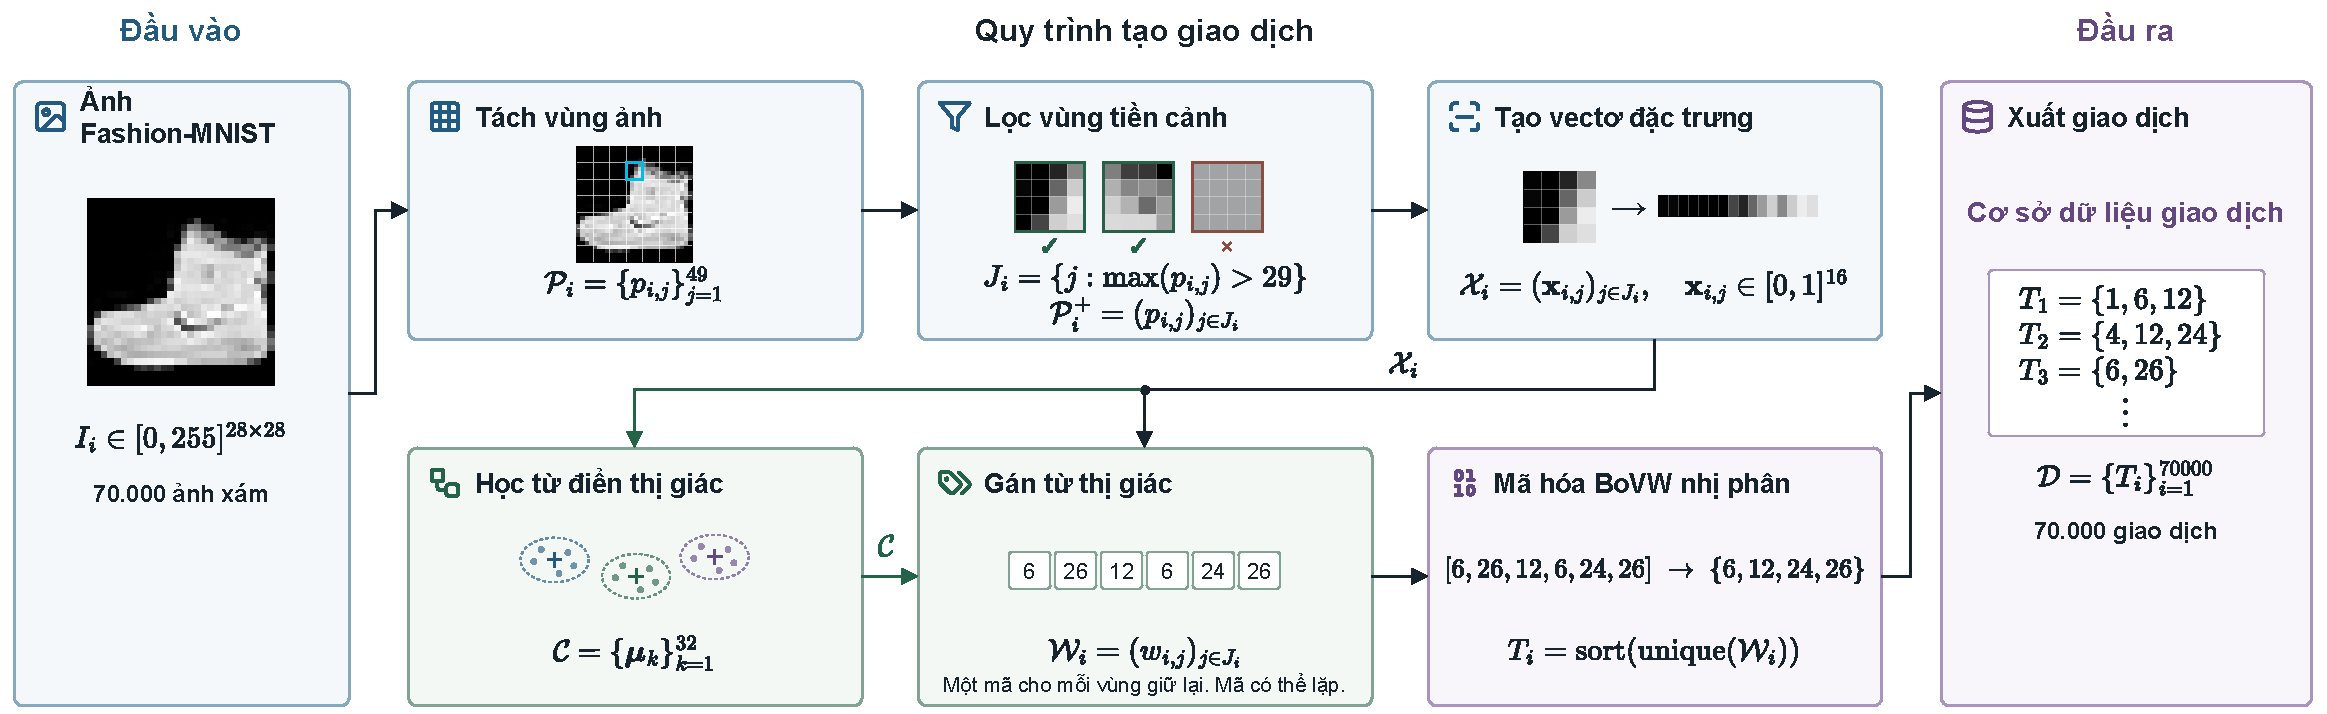
\includegraphics[width=0.98\textwidth]{TC_pipeline.pdf}
\caption{Quy trình dựng giao dịch từ ảnh. Các mã và giao dịch trong sơ đồ chỉ minh họa cấu trúc; TC4 release học một codebook chung từ toàn bộ 70.000 ảnh.}
\label{fig:fashion-pipeline}
\end{figure*}

Một patch $p$ được giữ khi
\begin{equation}
\max_{u,v}p_{u,v}>29.
\label{eq:foreground}
\end{equation}
Đây là điều kiện có ít nhất một pixel lớn hơn 29, không phải mean pixel
lớn hơn 29. Ngưỡng cố định và phép so sánh nghiêm ngặt phải giữ nguyên
giữa các run. Bộ lọc giảm vùng nền gần như đen; nó không bảo đảm mọi
patch còn lại có nghĩa như cổ áo hoặc đế giày.

Với patch giữ lại, descriptor $x_p\in[0,1]^{16}$ là
\begin{equation}
x_p=\frac{\operatorname{vec}(p)}{255},
\end{equation}
trong đó vec đọc 16 pixel theo thứ tự cột và lưu Float32. Thứ tự duyệt
patch trên ảnh và thứ tự flatten bên trong patch là hai quy ước khác
nhau. Dùng cùng quy ước khi reshape centroid về $4\times4$ để tránh đổi
vị trí pixel trong hình diễn giải.

Giả sử ảnh $i$ còn $q_i$ patch sau lọc, tổng descriptor là
$P=\sum_iq_i$, với $0\leq q_i\leq49$. Ma trận có shape $16\times P$.
Cần đối chiếu số cột với số hàng patch metadata, kiểm tra giá trị hữu hạn
và miền $[0,1]$. Không nối nhãn và tọa độ vào vector, vì chúng sẽ đổi
khoảng cách và ý nghĩa visual word đã chốt.

\subsubsection{TC4: học codebook bằng K-means}
B0 dùng K-means full-batch trên toàn bộ descriptors giữ lại, không lấy
mẫu ảnh hoặc descriptor trong profile release. Với $K=32$ centroid
$\mu_1,\ldots,\mu_K$, mục tiêu là giảm
\begin{equation}
J=\sum_{p=1}^{P}\min_{1\leq k\leq K}\|x_p-\mu_k\|_2^2.
\label{eq:kmeans}
\end{equation}
Vòng lặp gán cụm/cập nhật tâm theo K-means~\cite{lloyd} do
Clustering.jl thực hiện~\cite{clustering}; core FIM vẫn là Eclat tự cài
đặt. Khởi tạo dùng K-means++~\cite{kmpp} với seed 123.

\begin{reporttable}
\caption{Cấu hình codebook Fashion release; đây là tham số, không phải kết quả benchmark.}
\label{tab:fashion-config}
\small
\begin{tabular}{lp{0.52\columnwidth}}\toprule
Thuộc tính & Giá trị\\\midrule
Ảnh tham gia fit & Đủ 70.000 ảnh\\
Descriptor & Raw pixels, 16D Float32/255\\
Codebook & B0, full-batch K-means\\
Số cụm và seed & K=32, seed=123\\
Khởi tạo & K-means++\\
Giới hạn vòng lặp & 300\\
Tolerance & $10^{-4}$\\
Khoảng cách & Squared Euclidean\\\bottomrule
\end{tabular}
\end{reporttable}

Bảng~\ref{tab:fashion-config} xác định thí nghiệm phải tái lập. Seed cố
định ngẫu nhiên trong cùng môi trường, nhưng không thay việc ghi phiên
bản thư viện, kiểu số và artifact hash. Kiểm tra centroid shape
$16\times32$, giá trị hữu hạn, occupancy và trạng thái hội tụ. Chạm giới
hạn vòng lặp không được diễn giải như đã hội tụ.

K-means gộp các vùng có khoảng cách pixel nhỏ, nên visual word có thể là
kiểu chuyển tiếp sáng tối thay vì một bộ phận quần áo. Hai ảnh khác lớp
có thể dùng cùng từ; một vật thể cùng lớp có thể đổi mã khi thay độ sáng
hoặc vị trí biên. Đặt tên ngữ nghĩa cho word cần dựa trên patch thật,
không chỉ centroid.

\subsubsection{TC5--TC6: gán từ và mã hóa giao dịch}
Mỗi descriptor nhận mã tâm gần nhất:
\begin{equation}
w_p=\operatorname*{arg\,min}_{1\leq k\leq32}\|x_p-\mu_k\|_2^2.
\end{equation}
Nếu khoảng cách bằng nhau, cài đặt chọn ID nhỏ nhất. Giữ mapping từ mã
về image ID, patch ID và tọa độ. ID cluster không có thứ tự ngữ nghĩa;
word 10 không lớn hơn word 2 theo nghĩa đặc trưng.

Giao dịch S0 của ảnh $I_i$ là
\begin{equation}
T_i=\operatorname{sort}\!\left(\operatorname{unique}
 \{w_p:p\text{ thuộc }I_i\}\right).
\label{eq:s0}
\end{equation}
Mỗi word xuất hiện tối đa một lần trong giỏ. Binary BoVW bỏ qua số patch
lặp và vị trí tương đối. Support đếm số ảnh chứa đủ các word, không đếm
số patch hoặc số lần word xuất hiện.

Nếu không patch nào vượt bộ lọc, ảnh vẫn tạo một giao dịch rỗng. Bỏ ảnh
này sẽ đổi mẫu số support và phân bố lớp. Số giao dịch release phải bằng
70.000, mỗi TID có đúng một image ID. Không áp đặt mọi giao dịch đều
không rỗng nếu chưa đọc kết quả kiểm định.

Bất biến TC6 gồm item thuộc $1{:}32$, item tăng dần và duy nhất, số giao
dịch bằng số ảnh, TID/image ID không lặp. Hai transaction bằng nhau vẫn
là hai quan sát. Codebook và encoding phải cố định trước khi so backend;
fit lại K-means cho mỗi backend sẽ đổi đầu vào của phép so sánh.

\subsubsection{TC7: kiểm định artifact và truy vết}
TC7 đọc lại dữ liệu đã ghi, không chỉ kiểm tra biến trong bộ nhớ.
Bảng~\ref{tab:fashion-artifacts} liệt kê đầu vào của mining/diễn giải.
Manifest ghi run identity, configuration, số ảnh và SHA-256 để phát hiện
ghép nhầm centroid của một lần fit với transaction của lần khác.

\begin{reporttable}
\caption{Artifact truy vết Fashion; các đường dẫn thuộc cùng một run.}
\label{tab:fashion-artifacts}
\footnotesize
\begin{tabular}{lp{0.49\columnwidth}}\toprule
Artifact & Vai trò\\\midrule
Dataset manifest & Nguồn archive, split và hash\\
Transactions JSONL & Một dòng/TID, image ID, tập word\\
Codebook, centroids & Tâm cụm và không gian descriptor\\
Patch assignments & Word gán cho từng vùng ảnh\\
TID/image mapping & Liên kết giao dịch với ảnh nguồn\\
Image metadata & Split, source index và nhãn lớp\\
TC7 manifest & Kiểm định và hash các artifact\\\bottomrule
\end{tabular}
\end{reporttable}

Cùng số hàng chưa đủ xác nhận mapping đúng: thứ tự và ID phải khớp từng
bản ghi. Image ID phải tái tạo được từ split và index nguồn. Với một
hình minh họa, cần tìm được transaction, tọa độ patch và assignment
tương ứng. Gallery đẹp nhưng không nối được bằng chứng chưa xác nhận
được mẫu mined.

\subsubsection{Thiết kế khai thác và đối chiếu}
Hai backend dùng cùng file tại sáu ngưỡng Bảng~\ref{tab:fashion-thresholds}.
Nhãn không tham gia mining. Dùng cùng số luồng, giới hạn tài nguyên và
chính sách ghi output; không cho hai backend cạnh tranh tài nguyên khi đo.

\begin{reporttable}
\caption{Ngưỡng Fashion release trên mẫu số 70.000 ảnh.}
\label{tab:fashion-thresholds}
\small
\begin{tabular}{rr}\toprule
Minsup (\%) & Min-count\\\midrule
80 & 56.000\\60 & 42.000\\40 & 28.000\\
20 & 14.000\\10 & 7.000\\5 & 3.500\\\bottomrule
\end{tabular}
\end{reporttable}

Với itemset $X$, support được audit trực tiếp:
\begin{equation}
c(X)=\sum_{i=1}^{70000}\mathbf{1}[X\subseteq T_i].
\label{eq:fashion-audit}
\end{equation}
So mọi key và count giữa hai backend. Chỉ báo parity đạt khi cả hai run
hoàn tất và toàn bộ ánh xạ giống nhau. Bằng số lượng không thay thế phép
so này; zero kết quả hợp lệ khác với timeout chưa ghi xong file.

\begin{reporttable}
\caption{Kết quả Fashion 70k chờ cập nhật. S/BV là Set/BitVector, RSS tính bằng MiB; các số đo và parity của lần chạy này đều chưa được xác nhận.}
\label{tab:fashion-results}
\footnotesize
\begin{tabular}{rrrrrr}\toprule
$s$ (\%) & Itemsets & $t_S$ (s) & $t_{BV}$ (s) & RSS S/BV & Parity\\\midrule
80 & \pending & \pending & \pending & \pending & \pending\\
60 & \pending & \pending & \pending & \pending & \pending\\
40 & \pending & \pending & \pending & \pending & \pending\\
20 & \pending & \pending & \pending & \pending & \pending\\
10 & \pending & \pending & \pending & \pending & \pending\\
5 & \pending & \pending & \pending & \pending & \pending\\\bottomrule
\end{tabular}
\end{reporttable}

Bảng~\ref{tab:fashion-results} không điền số lịch sử 7.228 như một kết
quả mặc định. Chỉ so với số đó khi transaction hash trùng input của báo
cáo cũ; khác hash ghi không áp dụng. Min-count là tham số đã biết, còn
itemset count, runtime và RSS phải lấy từ artifact hoàn tất.

Đồ thị cần có số itemsets theo minsup, độ dài tối đa và phân bố độ dài,
runtime hai backend và Peak RSS nếu có phép đo hợp lệ. Một lượt mỗi
ngưỡng chỉ mô tả lần chạy đó, chưa chứng minh độ ổn định. Phạm vi đồng
hồ phải ghi rõ trước khi so với Chương II.

\subsubsection{Hai đường thực thi và tình trạng xác minh}
Bộ bốn notebook release nối dataset, transactions, mining và interpretation
bằng manifest. Supervisor dùng Linux user-systemd để giới hạn/theo dõi
worker, ghi trạng thái lỗi tài nguyên và Peak RSS. Run chưa hoàn tất
không được đổi thành parity đạt.

Demo Colab dùng Python kernel gọi Julia và chạy trực tiếp core. Profile
mẫu đã chạy với 1.000 ảnh; profile full gọi cấu hình dựng giao dịch release
70.000 ảnh. Demo đo riêng mine, không có Peak RSS của Fashion. Nó kiểm
tra parity/support, nhưng selection minh họa không thay hợp đồng selector
của Notebook 03--04. Không ghi RSS bằng 0 khi metric chưa đo.

Lần chạy full Colab mới chưa hoàn tất vì runtime bị thu hồi lúc chuẩn bị
môi trường, sau đó dịch vụ từ chối cấp phát tiếp. Điều này chưa xác nhận
lỗi thuật toán, nhưng cũng chưa xác nhận full workflow hoàn tất. Bảng 70k
vì vậy vẫn để trống. Khi cập nhật, ghi rõ đường demo hay bốn notebook
release; không suy từ mẫu nhỏ rằng full-data đã được nghiệm thu.

\subsubsection{Chọn mẫu đại diện}
Selector release gộp và loại trùng itemsets từ các run Set hoàn tất.
Cùng tập xuất hiện ở nhiều ngưỡng phải có support nhất quán; ngưỡng
nguồn là ngưỡng cao nhất đã quan sát. Chia kết quả theo độ dài 1, 2,
$\geq3$ và ba nhóm support thấp/vừa/cao.

Chia nhóm theo thứ hạng các support count phân biệt, để các mẫu cùng số
đếm không bị tách nhóm. Chọn trước từ ba ô (1/cao), (2/vừa), ($\geq3$/thấp)
nếu có ứng viên hợp lệ, rồi điền theo lưới chín ô cố định. Trong mỗi ô
ưu tiên support giảm dần, độ dài, rồi tuple item để không phụ thuộc Dict.

Độ trùng giữa hai mẫu dùng Jaccard:
\begin{equation}
J(X,Y)=\frac{|X\cap Y|}{|X\cup Y|}.
\end{equation}
Chọn tối đa bốn mẫu với ngưỡng 0,80; chưa đủ thì chạy lại một lần ở 0,90.
Bàn giao ba mẫu nếu không có mẫu thứ tư hợp lệ; ít hơn ba phải dừng.
Đây là quy tắc đa dạng hóa mẫu để review, không tối ưu chất lượng phân loại.

Manifest lựa chọn ghi phiên bản quy tắc, thứ tự mẫu, Jaccard, hash catalog
và output nguồn. Không sửa thủ công CSV rồi coi đó là output selector.
Chọn mẫu tự động khác với đánh giá ngữ nghĩa bằng người; trạng thái hai
bước phải được ghi riêng.

\subsubsection{Từ itemset về centroid, patch và ảnh}
Với mỗi word, reshape centroid về $4\times4$ theo thứ tự flatten đã dùng,
đặt cạnh patch thật được gán vào word đó. Giữ tọa độ witness để đánh dấu
vùng trên ảnh gốc. Centroid là trung bình trong không gian descriptor;
nhìn riêng centroid có thể bỏ qua khác biệt giữa các patch cùng cụm.

Với mẫu $X$, lấy toàn bộ ảnh có $X\subseteq T_i$ và kiểm tra số ảnh bằng
support đã audit. Hiển thị tối đa sáu ảnh hỗ trợ theo lựa chọn xác định
và một đối chứng thiếu ít nhất một word nếu có. Không có đối chứng thì
ghi rõ, không tạo ảnh giả.

\begin{reportfigure}
\pendingplot{42mm}{Gallery từ run 70k\\Centroids, patch thật và tọa độ witness\\Ảnh hỗ trợ và ảnh đối chứng}
\caption{Vị trí gallery sau khi có selection manifest và retrieval audit; chưa dùng hình lịch sử như bằng chứng cho run mới.}
\label{fig:fashion-gallery}
\end{reportfigure}

Hình~\ref{fig:fashion-gallery} cần cho thấy mẫu tạo bởi những vùng sáng/tối
nào, gặp ở lớp nào và có nhất quán qua nhiều ảnh không. S0 không giữ vị
trí tương đối, nên không suy ra bố cục lặp lại từ đồng xuất hiện. Nhận
xét về biên cổ áo cần patch/ảnh và reviewer, không thể suy từ word ID.

\begin{reporttable}
\caption{Mẫu 70k chờ lựa chọn/audit; chỉ điền hàng được selector bàn giao.}
\label{tab:fashion-patterns}
\footnotesize
\begin{tabular}{lrrrr}\toprule
Mẫu & Items & Count & Support & Lớp nổi bật\\\midrule
P1 & \pending & \pending & \pending & \pending\\
P2 & \pending & \pending & \pending & \pending\\
P3 & \pending & \pending & \pending & \pending\\
P4 (nếu có) & \pending & \pending & \pending & \pending\\\bottomrule
\end{tabular}
\end{reporttable}

Mỗi hàng Bảng~\ref{tab:fashion-patterns} phải nối tới output Eclat và image
IDs. Người review ghi mức rõ ràng của witness, tính nhất quán hình thái,
nhận xét và hạn chế. Trạng thái bắt đầu là chờ review; pipeline xuất hình
không tự chứng nhận mọi diễn giải đúng.

\subsubsection{Phân bố theo lớp và enrichment}
Sau mining mới nối giao dịch với class label qua stable image ID. Với
$n_c$ ảnh lớp $c$, đặt $c_c(X)$ là số ảnh lớp đó chứa $X$:
\begin{equation}
s_c(X)=\frac{c_c(X)}{n_c},\qquad
E(X,c)=\frac{s_c(X)}{c(X)/N}.
\label{eq:enrichment}
\end{equation}
Mọi ký hiệu dùng cùng run/mẫu số; full dataset có $n_c=7.000$. Kiểm tra
$\sum_c c_c(X)=c(X)$ để phát hiện lỗi mapping. Với support dương,
$E>1$ nghĩa là phổ biến hơn trong lớp so với mức chung, không phải xác
suất phân loại đúng.

Mẫu support cao có thể gặp ở nhiều lớp nên ít phân biệt; mẫu hiếm hơn
có thể tập trung vào một lớp nhưng kém độ phủ. Đọc cùng count, support
theo lớp và enrichment, không chỉ xếp theo $E$. Cùng itemset có thể có
$E\geq2$ cho nhiều lớp; nhiều itemsets có thể chia sẻ phần lớn words.

Bảng lớp/heatmap có thể cho thấy lớp nào chứa nhiều mẫu tập trung, nhưng
đó là phân tích hậu nghiệm. Không dùng nhãn chọn codebook rồi gọi mức
trùng khớp theo lớp là đánh giá độc lập. Nhận xét tổng quát cần ghi cả
quy tắc chọn và số mẫu đã xem.

\subsubsection{Khả năng sử dụng và giới hạn}
Một hướng tiếp theo là biến $m$ frequent itemsets $P_1,\ldots,P_m$ thành
đặc trưng nhị phân của ảnh $I_i$:
\begin{equation}
\phi_j(I_i)=\mathbf{1}[P_j\subseteq T_i],\quad j=1,\ldots,m.
\end{equation}
Các biến mô tả đồng xuất hiện nhiều words, có thể so với BoVW đơn lẻ
bằng cùng một classifier. Hướng đánh giá đề xuất là so BoVW, itemset
features và tổ hợp của chúng với accuracy/Macro-F1. Chưa có kết quả
classifier và không tuyên bố cải thiện.

Codebook release fit cả train và test gốc để mô tả 70.000 ảnh. Dùng
chính dữ liệu đó đánh giá dự đoán có thể gây thiên lệch. Thí nghiệm
classifier độc lập phải fit codebook, mine và chọn features trên train,
cố định phép biến đổi rồi mới áp lên test. Spatial encoding, PCA và
lượng tử hóa là hướng riêng, chưa phải bằng chứng tốt hơn của S0.

Raw descriptor nhạy với thay đổi pixel, không bất biến quay/tỉ lệ.
S0 bỏ vị trí và tần suất patch; bộ lọc nền có thể giữ nhiễu sáng nhỏ.
Giảm minsup tăng chi phí và số mẫu cần review, trong khi nhiều mẫu chỉ
khác một word. Cần nêu các giới hạn này thay vì coi mọi itemset phổ biến
là một bộ phận có nghĩa hoặc quy tắc nhận dạng quần áo.
